\paragraph{Forward-backward recursions and M-step updates.}
For reference, the Baum-Welch description in the main text is underpinned by the standard log-space recursions~\cite{rabiner1986introduction, bilmes1998gentle}.
Define the forward variable $\alpha_t(k) = \Prob(O_{1:t}, S_t = k \mid \mathcal{M})$ and the backward variable $\beta_t(k) = \Prob(O_{t+1:T} \mid S_t = k, \mathcal{M})$.
The log-space recursions are
\begin{align}
    \log \alpha_1(k) &= \log \pi_k + \log f_k(O_1), \label{eq:forward_init} \\
    \log \alpha_t(j) &= \underset{i}{\text{logsumexp}}\!\left(\log \alpha_{t-1}(i) + \log T_{ij}\right) + \log f_j(O_t), \quad t = 2, \ldots, T, \label{eq:forward} \\[4pt]
    \log \beta_T(k) &= 0, \label{eq:backward_init} \\
    \log \beta_t(i) &= \underset{j}{\text{logsumexp}}\!\left(\log T_{ij} + \log f_j(O_{t+1}) + \log \beta_{t+1}(j)\right), \quad t = T{-}1, \ldots, 1, \label{eq:backward}
\end{align}
where $\text{logsumexp}_i(x_i) = x_{\max} + \log \sum_i \exp(x_i - x_{\max})$.
The posterior state-occupancy $\gamma_t(k)$ and pair-occupancy $\xi_t(i, j)$ quantities are
\begin{equation}
    \gamma_t(k) = \frac{\alpha_t(k) \beta_t(k)}{\sum_j \alpha_t(j) \beta_t(j)}, \qquad
    \xi_t(i, j) = \frac{\alpha_t(i)\, T_{ij}\, f_j(O_{t+1})\, \beta_{t+1}(j)}{\sum_{m,n} \alpha_t(m)\, T_{mn}\, f_n(O_{t+1})\, \beta_{t+1}(n)},
    \label{eq:gamma_xi}
\end{equation}
and the closed-form M-step updates are
\begin{equation}
    \pi_k^{\text{new}} = \gamma_1(k),\quad
    \mu_k^{\text{new}} = \frac{\sum_t \gamma_t(k)\, O_t}{\sum_t \gamma_t(k)},\quad
    \left(\sigma_k^{\text{new}}\right)^2 = \frac{\sum_t \gamma_t(k)(O_t - \mu_k^{\text{new}})^2}{\sum_t \gamma_t(k)},\quad
    T_{ij}^{\text{new}} = \frac{\sum_{t=1}^{T-1} \xi_t(i, j)}{\sum_{t=1}^{T-1} \gamma_t(i)}.
    \label{eq:mstep}
\end{equation}
The convergence criterion is $|\mathcal{L}^{(n)} - \mathcal{L}^{(n-1)}| < \epsilon$ with $\epsilon = 10^{-4}$, where $\mathcal{L}^{(n)} = \text{logsumexp}_k \log \alpha_T(k)$ is the standard Baum-Welch observed-data log-likelihood of the parameters entering iteration $n$, evaluated by that iteration's forward pass \emph{before} any M-step can mutate them; the check runs before the update, so the returned parameters are always an evaluated iterate with a matching smoothed posterior, and the loop makes one final evaluation-only pass so that the last M-step update is itself scored. For the exact Gaussian and Laplace conditional maximisations the likelihood is monotone across iterations and the last evaluated iterate is returned; for the Student-$t$ and GED numerical block updates ascent is not guaranteed, the trace is monitored instead (see the numerical-optimisation scope paragraph of the supplementary propositions), and the best evaluated finite iterate $\arg\max_n \mathcal{L}^{(n)}$ is returned. Implementation note on $\boldsymbol\pi$: the Gaussian fitter departs from Eq.~\eqref{eq:mstep} in one place, holding $\boldsymbol\pi$ fixed at its uniform initial value instead of applying $\pi_k^{\text{new}} = \gamma_1(k)$; the Student-$t$, Laplace, and GED fitters apply the $\gamma_1$ update. Parameter counts and BIC penalties for CHMM-N accordingly exclude $\boldsymbol\pi$. Simulation draws $S_1$ from the stationary distribution $\bar{\boldsymbol\pi}$ of $\hat{\mathbf T}$ and then iterates $G_t \sim \mathcal{N}(\mu_{S_t}, \sigma_{S_t}^2)$, $S_{t+1} \sim \text{Categorical}(\mathbf{T}_{S_t, \cdot})$ with no jump process.

\paragraph{CHMM-t M-step (per-state ECM/ECME, closed form given $u_{t,k}$).}
For Student-t emissions $f_k(x) = t_{\nu_k}(x; \mu_k, \sigma_k)$ the ECM formulation of \citet{peel2000robust, liu1995ml} treats the latent precision as an augmented E-step quantity,
\begin{equation}
    u_{t,k} = \frac{\nu_k + 1}{\nu_k + ((O_t - \mu_k)/\sigma_k)^2},
    \label{eq:tprecision_supp}
\end{equation}
so that conditional on $\nu_k$ the location and scale admit closed-form weighted updates,
\begin{equation}
    \mu_k^{\text{new}} = \frac{\sum_t \gamma_t(k)\, u_{t,k}\, O_t}{\sum_t \gamma_t(k)\, u_{t,k}},\quad
    \left(\sigma_k^{\text{new}}\right)^2 = \frac{\sum_t \gamma_t(k)\, u_{t,k}\, (O_t - \mu_k^{\text{new}})^2}{\sum_t \gamma_t(k)}.
    \label{eq:tupdate_supp}
\end{equation}
The degrees-of-freedom parameter $\nu_k$ is then refined by a 40-iteration one-dimensional golden-section search on the per-state posterior-weighted objective $Q_k(\nu) = \sum_t \gamma_t(k)\, \log t_\nu(O_t; \mu_k, \sigma_k)$ over the bracket $(\nu_{\min}, \nu_{\max}) = (2.1, 50)$, with the smoothed posteriors $\gamma$ held fixed. Maximising this marginal state-weighted log-likelihood for $\nu_k$, rather than the augmented-data $u$-functional, follows the spirit of the ECME construction of \citet{liu1995ml}; in their single-component i.i.d.\ setting, where all $\gamma_t(k) = 1$, that objective is the observed-data likelihood, whereas already for i.i.d.\ mixtures the posterior-weighted objective differs from the observed-data likelihood \citep{peel2000robust}, and in the HMM the observed-data likelihood also depends on $\nu_k$ through the forward recursion, so this update is a hybrid generalised block-coordinate step on a surrogate objective and does not inherit the ECME observed-data ascent guarantee. We diagnose convergence from the observed-data log-likelihood trace rather than assert monotonicity, returning the best evaluated finite iterate (which is also restored if an update degenerates to a non-finite likelihood).
We extend this M-step with an optional exponential shrinkage prior on $1/\nu_k$, corresponding to the penalised objective
\begin{equation}
    Q_k^{\text{pen}}(\nu) \;=\; \sum_t \gamma_t(k)\, \log t_\nu(O_t; \mu_k, \sigma_k) \;-\; \lambda \, / \, \nu,
    \label{eq:nu_pen}
\end{equation}
maximised by the same golden-section search ($\lambda = 0$ recovers the unpenalised \citet{peel2000robust, liu1995ml}-style $\nu$ update; the rate sweep and its effect on simulated IS excess kurtosis are reported in the $K$-selection and $\nu_k$ diagnostics appendix, Table~\ref{tab:nu_shrinkage}).

\paragraph{CHMM-L M-step (closed-form weighted Laplace MLE).}
For Laplace emissions $f_k(x) = \tfrac{1}{2 b_k} \exp(-|x - \mu_k|/b_k)$, with the per-state Laplace scale denoted $b_k$ to avoid collision with the backward variable $\beta_t$, the weighted-MLE estimators are available in closed form:
\begin{equation}
    \mu_k^{\text{new}} = \text{WeightedMedian}\!\left(O_{1:T};\, \gamma_{1:T}(k)\right),\qquad
    b_k^{\text{new}} = \frac{\sum_t \gamma_t(k)\, |O_t - \mu_k^{\text{new}}|}{\sum_t \gamma_t(k)}.
    \label{eq:lupdate_supp}
\end{equation}
The weighted median is the first order statistic whose cumulative posterior weight reaches half the total, the minimiser of the weighted $L^1$ objective $\sum_t \gamma_t(k)\,|O_t - \mu|$; when the half-weight falls exactly between two adjacent order statistics, every point in the closed interval between them is a minimiser.
The Laplace M-step carries no shape parameter, so CHMM-L is strictly cheaper per iteration than CHMM-t (which requires the per-state $Q_k$ search).

\paragraph{CHMM-GED M-step (three-stage ECM-style update with closed-form scale).}
For Generalized Error Distribution emissions $f_k(x) = \mathrm{GED}(x; \mu_k, \alpha_k, p_k) = \frac{p_k}{2 \alpha_k \Gamma(1/p_k)} \exp\!\big(-(|x - \mu_k|/\alpha_k)^{p_k}\big)$ the M-step decomposes into three block updates per state. Given current $(\mu_k^{(n)}, \alpha_k^{(n)}, p_k^{(n)})$, the first block updates the location by minimising the per-state weighted $L^{p_k}$ loss,
\begin{equation}
    \mu_k^{(n+1)} \;=\; \operatorname{GoldenSearchMin}_{\mu \in I_k} \;\sum_t \gamma_t(k)\, \big|O_t - \mu\big|^{p_k^{(n)}},
    \qquad I_k \;=\; \big[\min_t O_t,\, \max_t O_t\big],
    \label{eq:ged_mu}
\end{equation}
by a $40$-iteration golden-section search; CM-2 updates the scale in closed form given $(\mu_k^{(n+1)}, p_k^{(n)})$,
\begin{equation}
    \alpha_k^{(n+1)} \;=\; \left[\frac{p_k^{(n)}}{W_k} \sum_t \gamma_t(k)\, \big|O_t - \mu_k^{(n+1)}\big|^{p_k^{(n)}}\right]^{1 / p_k^{(n)}}, \qquad W_k \;=\; \sum_t \gamma_t(k);
    \label{eq:ged_alpha}
\end{equation}
and CM-3 updates the shape by maximising the per-state $Q$-function over the bracket,
\begin{equation}
    p_k^{(n+1)} \;=\; \operatorname{GoldenSearchMax}_{p \in [p_{\min},\, p_{\max}]} \;\sum_t \gamma_t(k)\, \log f_k\!\big(O_t;\, \mu_k^{(n+1)},\, \alpha_k^{(n+1)},\, p\big),
    \label{eq:ged_p}
\end{equation}
again by a $40$-iteration golden-section search over $[p_{\min}, p_{\max}] = [0.5, 3.0]$. The scale update is the exact conditional maximiser. The location objective is convex when $p_k \ge 1$ but can be nonconvex when $p_k < 1$, and both bracketed searches are finite numerical approximations. Accordingly, we use ``ECM-style'' for this three-block procedure and assess convergence from the observed-data log-likelihood trace; the exact ECM monotonicity result~\citep{mengrubin1993ecm} would require every block to attain a conditional maximum. At the boundary cases, $p_k = 2$ recovers Gaussian (with $\sigma = \alpha/\sqrt{2}$) and $p_k = 1$ recovers Laplace (with $b = \alpha$).

\paragraph{Algorithm descriptions.}
The unified EM procedure shared across all four emission families is given in Algorithm~\ref{alg:chmm_em}: a shared framework (quantile-based initialisation, log-space forward-backward, transition update) plus four family-specific branches at lines~\ref{line:init}, \ref{line:emit}, and \ref{line:mstep}. The simulator is given in Algorithm~\ref{alg:chmm_simulate}, and the cross-asset rank-reordering simulator for the multi-asset construction in Algorithm~\ref{alg:copula_sim}. Viterbi and SIM-resampling pseudocode are provided in the companion code repository; both are textbook constructions and we omit them from the appendix.

% ========================================================================================= %
% Algorithm 1: Baum-Welch (EM) for Continuous Gaussian HMM
% ========================================================================================= %
% Unified EM algorithm with family-specific M-step switch
% ========================================================================================= %
\begin{breakablealgorithm}
\caption{Unified EM algorithm for the CHMM family. Lines~\ref{line:init}, \ref{line:emit}, and \ref{line:mstep} branch on the emission family $F \in \{\mathcal{N}, t, L, \text{GED}\}$; every other line is identical across families. The CHMM-N and CHMM-L variants instantiate classical EM; CHMM-t and CHMM-GED use ECM-style block updates whose shape step is a finite one-dimensional golden-section search. Hyperparameter defaults used throughout this paper: convergence tolerance $\epsilon = 10^{-4}$ on $\Delta \mathcal L$, $\texttt{max\_iter} = 60$, $40$-iteration golden-section sub-step on every bracketed update, CHMM-t bracket $(\nu_{\min}, \nu_{\max}) = (2.1, 50)$ with initial $\nu^{(0)} = 6$, CHMM-GED bracket $(p_{\min}, p_{\max}) = (0.5, 3.0)$ with initial $p^{(0)} = 1.5$ and a $\mu_k$ search interval widened to cover the observed data range.}
\label{alg:chmm_em}
\footnotesize
\setlength{\baselineskip}{0.95\baselineskip}
\begin{algorithmic}[1]
\REQUIRE Observations $O_{1:T}$, number of states $K$, tolerance $\epsilon$, $\texttt{max\_iter}$, emission family $F \in \{\mathcal{N}, t, L, \text{GED}\}$, if $F = t$ bracket $(\nu_{\min}, \nu_{\max})$ and initial $\nu^{(0)}$, if $F = \text{GED}$ bracket $(p_{\min}, p_{\max})$ and initial $p^{(0)}$.
\ENSURE Transition matrix $\mathbf{T}$, per-state emission parameters $\boldsymbol\theta_{1:K}$, initial distribution $\boldsymbol{\pi}$.

\STATE \textbf{Quantile-Based Initialization.}
\STATE Sort $O^{(\text{sort})} \leftarrow \text{sort}(O_{1:T})$ and partition into $K$ equal chunks $\{C_1,\ldots,C_K\}$.
\FOR{$k = 1$ to $K$} \label{line:init}
    \STATE \textbf{switch} $F$
    \STATE \quad $F = \mathcal{N}$: $\mu_k \leftarrow \text{mean}(C_k)$, \quad $\sigma_k \leftarrow \max(\text{std}(C_k), 10^{-6})$.
    \STATE \quad $F = t$: $\mu_k \leftarrow \text{mean}(C_k)$, \quad $\sigma_k \leftarrow \max(\text{std}(C_k), 10^{-6})$, \quad $\nu_k \leftarrow \nu^{(0)}$.
    \STATE \quad $F = L$: $\mu_k \leftarrow \text{median}(C_k)$, \quad $b_k \leftarrow \max(\text{mean}(|C_k - \mu_k|), 10^{-6})$. \COMMENT{Laplace scale $b_k$.}
    \STATE \quad $F = \text{GED}$: $\mu_k \leftarrow \text{mean}(C_k)$, \quad $\alpha_k \leftarrow \max(\text{std}(C_k), 10^{-6})$, \quad $p_k \leftarrow p^{(0)}$.
\ENDFOR
\STATE $T_{ij} \leftarrow 1/K$; \quad $\pi_k \leftarrow 1/K$; \quad $\mathcal{L}_{\text{prev}} \leftarrow -\infty$.

\STATE \textbf{EM Loop.} \COMMENT{one final evaluation-only pass, so every returned iterate has an evaluated likelihood.}
\FOR{$n = 1$ to $\texttt{max\_iter} + 1$}

    \STATE \textbf{E-Step, per-family emission log-likelihood.} \label{line:emit}
    \STATE \textbf{switch} $F$
    \STATE \quad $F = \mathcal{N}$: $\log B_{t,k} \leftarrow \log \mathcal{N}(O_t \mid \mu_k, \sigma_k^2)$.
    \STATE \quad $F = t$: $\log B_{t,k} \leftarrow \log t_{\nu_k}(O_t; \mu_k, \sigma_k)$.
    \STATE \quad $F = L$: $\log B_{t,k} \leftarrow -\log(2 b_k) - |O_t - \mu_k|/b_k$.
    \STATE \quad $F = \text{GED}$: $\log B_{t,k} \leftarrow \log p_k - \log(2 \alpha_k) - \log \Gamma(1/p_k) - (|O_t - \mu_k|/\alpha_k)^{p_k}$.

    \STATE \textbf{E-Step, shared log-space forward-backward.}
    \STATE $\log \alpha_1(k) \leftarrow \log \pi_k + \log B_{1,k}$.
    \FOR{$t = 2$ to $T$, $j = 1$ to $K$}
        \STATE $\log \alpha_t(j) \leftarrow \underset{i}{\text{logsumexp}}\!\left(\log \alpha_{t-1}(i) + \log T_{ij}\right) + \log B_{t,j}$.
    \ENDFOR
    \STATE $\log \beta_T(k) \leftarrow 0$.
    \FOR{$t = T-1$ down to $1$, $i = 1$ to $K$}
        \STATE $\log \beta_t(i) \leftarrow \underset{j}{\text{logsumexp}}\!\left(\log T_{ij} + \log B_{t+1,j} + \log \beta_{t+1}(j)\right)$.
    \ENDFOR
    \STATE Compute $\gamma_t(k)$ and $\xi_t(i,j)$ from equation~\eqref{eq:gamma_xi}.

    \STATE \textbf{Likelihood of the current iterate.} $\mathcal{L}^{(n)} \leftarrow \underset{k}{\text{logsumexp}}(\log \alpha_T(k))$ \COMMENT{observed-data log-likelihood of the parameters entering iteration $n$, evaluated before any update; for $F \in \{t, \text{GED}\}$ record $(\text{parameters}, \mathcal{L}^{(n)}, \gamma)$ as the best checkpoint whenever $\mathcal{L}^{(n)}$ improves on it.}
    \IF{$|\mathcal{L}^{(n)} - \mathcal{L}_{\text{prev}}| < \epsilon$ \textbf{ or } $n = \texttt{max\_iter} + 1$} \STATE \textbf{break} \COMMENT{the just-evaluated iterate is returned; no unevaluated update can escape the loop.} \ENDIF
    \STATE $\mathcal{L}_{\text{prev}} \leftarrow \mathcal{L}^{(n)}$.

    \STATE \textbf{Shared transition update.} $T_{ij} \leftarrow \sum_{t=1}^{T-1} \xi_t(i,j) \;/\; \sum_{t=1}^{T-1} \gamma_t(i)$; \quad $\pi_k \leftarrow \gamma_1(k)$ for $F \in \{t, L, \text{GED}\}$ \COMMENT{both sums run over $t = 1, \ldots, T-1$, one fewer term than the $\gamma$ sums of the emission updates below; for $F = \mathcal{N}$, $\boldsymbol\pi$ stays at its uniform initial value by documented convention.}

    \STATE \textbf{M-Step, per-family emission update.} \label{line:mstep}
    \STATE \textbf{switch} $F$
    \STATE \quad $F = \mathcal{N}$ \COMMENT{classical Baum-Welch~\citep{baum1970maximization}.}
    \STATE \qquad $\mu_k \leftarrow \sum_t \gamma_t(k)\, O_t / \sum_t \gamma_t(k)$.
    \STATE \qquad $\sigma_k \leftarrow \max\!\left(\sqrt{\sum_t \gamma_t(k) (O_t - \mu_k)^2 / \sum_t \gamma_t(k)},\; 10^{-6}\right)$.
    \STATE \quad $F = t$ \COMMENT{ECM-style block updates after \citet{peel2000robust, liu1995ml}; closed-form $(\mu_k, \sigma_k)$ given $\nu_k$, then 1D search on $\nu_k$ at fixed $\gamma$.}
    \STATE \qquad $u_{t,k} \leftarrow (\nu_k + 1) / (\nu_k + ((O_t - \mu_k)/\sigma_k)^2)$ for all $t, k$.
    \STATE \qquad $\mu_k \leftarrow \sum_t \gamma_t(k)\, u_{t,k}\, O_t / \sum_t \gamma_t(k)\, u_{t,k}$.
    \STATE \qquad $\sigma_k \leftarrow \max\!\left(\sqrt{\sum_t \gamma_t(k)\, u_{t,k}\,(O_t - \mu_k)^2 / \sum_t \gamma_t(k)},\; 10^{-6}\right)$.
    \STATE \qquad $\nu_k \leftarrow \operatorname{GoldenSearchMax}_{\nu \in [\nu_{\min}, \nu_{\max}]} \sum_t \gamma_t(k)\, \log t_\nu(O_t; \mu_k, \sigma_k)$ \COMMENT{40 iterations.}
    \STATE \quad $F = L$ \COMMENT{closed-form weighted Laplace MLE.}
    \STATE \qquad $\mu_k \leftarrow \text{WeightedMedian}(O_{1:T},\, \gamma_{1:T}(k))$ \COMMENT{first order statistic with cumulative weight $\ge W_k/2$.}
    \STATE \qquad $b_k \leftarrow \max\!\left(\sum_t \gamma_t(k)\, |O_t - \mu_k| / \sum_t \gamma_t(k),\; 10^{-6}\right)$.
    \STATE \quad $F = \text{GED}$ \COMMENT{three-stage ECM-style update: bracketed $\mu_k$, closed-form $\alpha_k$, bracketed $p_k$.}
    \STATE \qquad $\mu_k \leftarrow \operatorname{GoldenSearchMin}_{\mu \in I_k} \sum_t \gamma_t(k)\, |O_t - \mu|^{p_k}$ \COMMENT{40 iterations on $I_k = [\min_t O_t, \max_t O_t]$.}
    \STATE \qquad $\alpha_k \leftarrow \max\!\Big(\big[(p_k / W_k) \sum_t \gamma_t(k)\, |O_t - \mu_k|^{p_k}\big]^{1/p_k},\; 10^{-6}\Big)$ where $W_k = \sum_t \gamma_t(k)$ \COMMENT{closed form, unique zero of $\partial Q_k / \partial \alpha$.}
    \STATE \qquad $p_k \leftarrow \operatorname{GoldenSearchMax}_{p \in [p_{\min}, p_{\max}]} \sum_t \gamma_t(k)\, \log \mathrm{GED}(O_t; \mu_k, \alpha_k, p)$ \COMMENT{40 iterations.}
\ENDFOR

\RETURN $\mathbf{T}, \boldsymbol\theta_{1:K}, \boldsymbol{\pi}$ \COMMENT{$\boldsymbol\theta_k = (\mu_k, \sigma_k)$ for $F = \mathcal{N}$; $(\mu_k, \sigma_k, \nu_k)$ for $F = t$; $(\mu_k, b_k)$ for $F = L$; $(\mu_k, \alpha_k, p_k)$ for $F = \text{GED}$. For $F \in \{\mathcal{N}, L\}$ the last evaluated iterate is returned (EM ascent is exact for these families); for $F \in \{t, \text{GED}\}$, whose hybrid surrogate blocks do not guarantee observed-data ascent, the best evaluated finite checkpoint $\arg\max_n \mathcal{L}^{(n)}$ is returned, and a non-finite forward pass restores that checkpoint as well. In all cases the returned parameters carry an evaluated likelihood and a matching posterior $\gamma$.}
\end{algorithmic}
\end{breakablealgorithm}

% Viterbi pseudocode omitted (textbook construction; reference implementation in companion code repository).

% ========================================================================================= %
% Algorithm 3: CHMM Simulation
% ========================================================================================= %
\begin{algorithm}[tp]
\caption{CHMM simulation of synthetic excess growth rate paths (unified four-family framework). The emission draw at line~\ref{line:simemit} branches on the family $F \in \{\mathcal{N}, t, L, \text{GED}\}$ exactly as in Algorithm~\ref{alg:chmm_em}: $\mathcal{N}(\mu_k, \sigma_k^2)$ for CHMM-N, $t_{\nu_k}(\mu_k, \sigma_k)$ for CHMM-t, $\mathrm{Laplace}(\mu_k, b_k)$ for CHMM-L, $\mathrm{GED}(\mu_k, \alpha_k, p_k)$ for CHMM-GED; the latent chain and transition step are shared.}
\label{alg:chmm_simulate}
\small
\begin{algorithmic}[1]
\REQUIRE Trained CHMM $\mathcal{M} = (\mathbf{T}, \{\boldsymbol\theta_k\}, \boldsymbol{\pi}, F)$ with $\boldsymbol\theta_k = (\mu_k, \sigma_k)$ for $F = \mathcal{N}$; $(\mu_k, \sigma_k, \nu_k)$ for $F = t$; $(\mu_k, b_k)$ for $F = L$; $(\mu_k, \alpha_k, p_k)$ for $F = \mathrm{GED}$. Number of steps $M$, Number of paths $P$
\ENSURE Simulated growth-rate paths $\{\hat{G}^{(p)}_{1:M}\}_{p=1}^{P}$

\FOR{$p = 1$ to $P$}
    \STATE Sample initial state $S_1$ from the stationary distribution of $\hat{\mathbf T}$.
    \FOR{$t = 1$ to $M$}
        \STATE Emit observation $\hat{G}_t^{(p)} \sim f_{S_t}(\,\cdot\,;\, \boldsymbol\theta_{S_t})$ with $f_k$ the $F$-family per-state density. \label{line:simemit}
        \IF{$t < M$}
            \STATE Transition to next state $S_{t+1} \sim \text{Categorical}(\mathbf{T}_{S_t, \cdot})$.
        \ENDIF
    \ENDFOR
\ENDFOR

\RETURN $\{\hat{G}^{(p)}_{1:M}\}_{p=1}^{P}$
\end{algorithmic}
\end{algorithm}

% ========================================================================================= %
% Algorithm 4: Cross-Asset Copula Rank Reordering Simulation
% ========================================================================================= %
\begin{algorithm}[tp]
\caption{Cross-asset copula simulation via rank reordering}
\label{alg:copula_sim}
\small
\begin{algorithmic}[1]
\REQUIRE Fitted per-asset CHMMs $\{\mathcal{M}_j\}_{j=1}^d$, correlation matrix $\Sigma$ (positive semi-definite (PSD), unit diagonal), copula family $\mathcal{C} \in \{\text{Gaussian}, t_\nu\}$, path length $T$, number of paths $P$
\ENSURE Cross-asset path tensor $\{\hat{G}^{(p)}_{j,t}\}$ of shape $T \times d \times P$

\FOR{$p = 1$ to $P$}

    \STATE Draw copula sample $\mathbf{U}^{(p)} \in [0,1]^{T \times d}$ from $\mathcal{C}(\Sigma)$:
    \STATE \quad $L \leftarrow \text{Cholesky}(\Sigma)$, \; $Z \in \mathbb{R}^{T \times d} \sim \mathcal{N}(0, I_d)$ i.i.d.
    \STATE \quad $Y \leftarrow Z L^\top$
    \IF{$\mathcal{C} = $ Gaussian}
        \STATE \quad $\mathbf{U}^{(p)} \leftarrow \Phi(Y)$ componentwise
    \ELSE
        \STATE \quad Draw $W \sim \chi^2_\nu / \nu$ i.i.d. for $t = 1, \dots, T$; \; $X_{t,\cdot} \leftarrow Y_{t,\cdot} / \sqrt{W_t}$
        \STATE \quad $\mathbf{U}^{(p)} \leftarrow t_\nu(X)$ componentwise
    \ENDIF

    \FOR{$j = 1$ to $d$}
        \STATE Simulate $\tilde{g}_{j,1:T}^{(p)}$ from $\mathcal{M}_j$ via Algorithm~\ref{alg:chmm_simulate}.
        \STATE Compute order statistics $\tilde{g}_{j,(1)}^{(p)} \leq \cdots \leq \tilde{g}_{j,(T)}^{(p)}$.
        \STATE Compute ranks $r_{j,t}^{(p)} \leftarrow \text{rank}(U_{j,t}^{(p)})$ for $t = 1, \dots, T$.
        \STATE $\hat{G}_{j,t}^{(p)} \leftarrow \tilde{g}_{j,(r_{j,t}^{(p)})}^{(p)}$ for $t = 1, \dots, T$.
    \ENDFOR
\ENDFOR

\RETURN $\{\hat{G}^{(p)}_{j,t}\}$
\end{algorithmic}
\end{algorithm}

Scope remark on Algorithm~\ref{alg:copula_sim}: the copula sample $\mathbf{U}^{(p)}$ is drawn independently across the $T$ rows, so step 4 assigns each asset's sorted CHMM values to i.i.d.\ time ranks. Each column of the output is a permutation of the corresponding simulated CHMM path: the per-asset empirical marginal is preserved exactly and the contemporaneous cross-asset rank dependence follows $\mathcal{C}(\Sigma)$, but the per-asset serial dependence of the underlying CHMM path (volatility clustering, regime residence) is destroyed by the reordering. The output is a cross-sectional object, and the cross-asset evaluation accordingly scores per-asset marginal fit and cross-asset correlation reproduction only.

% SIM pseudocode omitted (standard rank-one factor regression with bootstrap residual resampling;
% reference implementation in companion code repository).


\paragraph{Per-state shape diagnostics: CHMM-t and CHMM-GED.}
This appendix backs the main-text discussion of the per-state shape allocation under CHMM-t and CHMM-GED on SPY IS at $K = 18$ (seed = $20260420$).

\paragraph{CHMM-t per-state $\nu_k$.}
The per-state $\nu_k$ histogram for the $K = 18$ CHMM-t fit is plotted in Figure~\ref{fig:nu_hist}.
Thirteen of the eighteen states rested at the upper ECM bracket ($\nu_k = 50$), and only two states lay near the lower bracket ($\nu_2 = 2.19$, $\nu_4 = 2.10$).
The simulated IS mixture excess kurtosis was driven by the posterior mass routed to those two very heavy-tailed states, not by a systemic collapse to the lower bracket.

\begin{figure}[!ht]
\centering
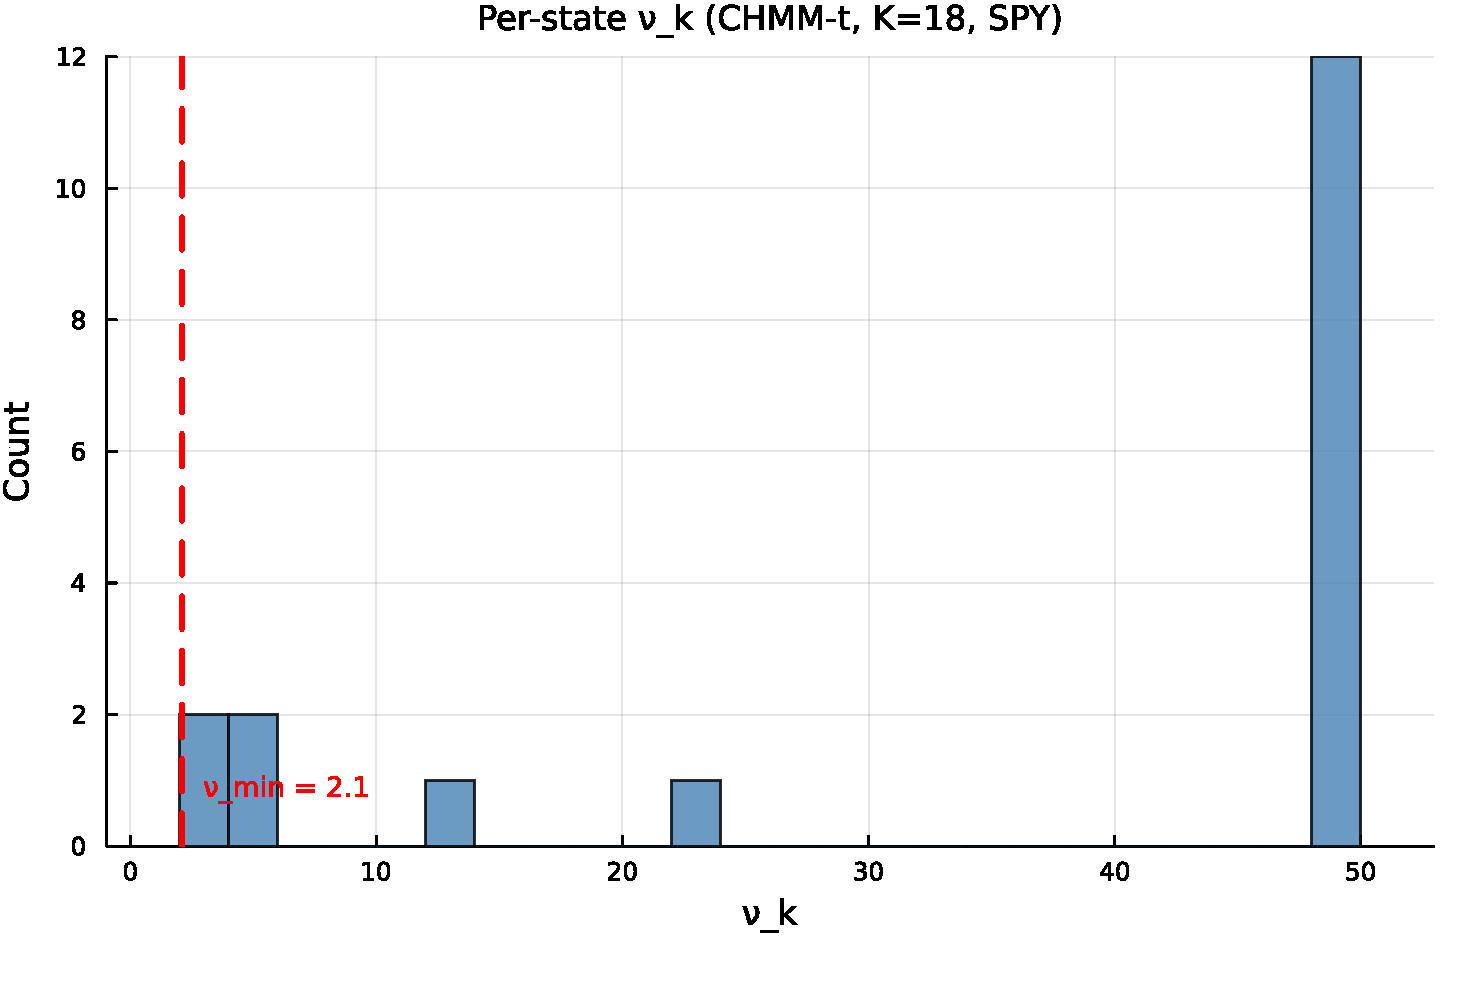
\includegraphics[width=0.65\textwidth]{figs/Fig-nu-Histogram.pdf}
\caption{Per-state degrees-of-freedom $\nu_k$ for the CHMM-t fit at $K = 18$ on SPY IS. The dashed red line marks the lower ECM bracket $\nu_{\min} = 2.1$. Only two states ($\nu_2 = 2.19$, $\nu_4 = 2.10$) sit near the lower bracket; the median $\nu_k$ is at the upper bracket.}
\label{fig:nu_hist}
\end{figure}

\paragraph{CHMM-GED per-state $p_k$ (Gaussian-bulk / Laplace-tail bimodality).}
The generator comparison reports and discusses the $\hat p_k$ partition (Figure~\ref{fig:p_hist}). Briefly, the $K = 18$ CHMM-GED fit on SPY IS was bimodal: eleven states attained exactly $p_k = 3.0$ (thirteen were Gaussian-like with $p_k \ge 1.85$), one state landed at intermediate $p_k = 1.6$, and four states clustered in the Laplace-shape regime $p_k \in [0.86, 1.24]$, concentrated in the high-volatility ranks. The smallest fitted $p_k$ on SPY was $0.86$, well clear of every $p_{\min}$ tested in the bracket sweep, so the lower bracket was non-binding. The bimodal partition replicated across $10$ Monte Carlo seeds and across the cross-asset universe (full robustness panel in the cross-asset robustness appendix).

\paragraph{Bracket-sensitivity sweeps.}
A CHMM-t bracket sweep on $\nu_{\min} \in \{2.1, 2.5, 3.0, 4.0, \infty\}$ at $K = 18$ showed that the excess kurtosis overshoot is a feature of the Student-$t$ emission at $K = 18$, not a lower-bracket artefact. The simulated IS excess kurtosis stayed in a heavy-tailed band across finite brackets and collapsed only in the full Gaussian limit. The analogous CHMM-GED sweep on $p_{\max} \in \{2.0, 2.5, 3.0, 3.5, 4.0\}$ left the non-Gaussian state count invariant, with Laplace-like states in $\{3,4,5\}$; tightening $p_{\max}$ from $4.0$ to $3.0$ cost only a few nats of LL. The $p_{\min}$ sweep on $\{0.5, 0.7, 0.85\}$ was fully degenerate: every floor produced an identical fit because the smallest observed $\hat p_k$ on SPY was $0.86$.


\paragraph{Evaluation summary.}
Observed growth rates $G_t$ are fit by Baum-Welch CHMM at the default $K^\star = 3$, with $K = 18$ retained as the sensitivity reference for excess kurtosis fidelity; $1{,}000$ paths are then simulated and per-asset metrics computed (Table~\ref{tab:model_comparison}). For the multi-asset analysis we reuse the per-asset $K^\star = 3$ fits as marginals, draw a copula sample $\mathbf U \sim \mathcal C(\Sigma)$ from the fitted Student-$t$ copula on ranks, rank-reorder the per-asset single-asset paths to match $\mathbf U$, and report cross-asset metrics (Table~\ref{tab:cross_asset}). The single-asset CHMM framework is shared across both; the CHMM training and simulation steps are Algorithms~\ref{alg:chmm_em} and~\ref{alg:chmm_simulate}, the cross-asset rank-reordering step is Algorithm~\ref{alg:copula_sim}, and the architecture diagram for the single-asset framework is Figure~\ref{fig:chmm_architecture}.
